% Initial research manuscript, NOT peer reviewed, EXPLORATORY, Phase 2 (local, macOS) results only.
% NOT COMPILED: no LaTeX toolchain was available on the authoring machine (see COMPILE_OVERLEAF.md).
% If ieeeaccess.cls is installed, replace the documentclass line with \documentclass{ieeeaccess}; content files are class-independent.
\documentclass[journal]{IEEEtran}
\usepackage{cite}
\usepackage{amsmath,amssymb}
\usepackage{graphicx}
\usepackage{url}
\usepackage{xcolor}
\usepackage{array}
\usepackage{hyperref}
\def\BibTeX{{\rm B\kern-.05em{\sc i\kern-.025em b}\kern-.08em T\kern-.1667em\lower.7ex\hbox{E}\kern-.125em X}}
\newcommand{\NDO}{\texttt{NO\_DIVERGENCE\_OBSERVED}}
\newcommand{\DIV}{\texttt{DIVERGENT\_OBSERVABLE}}
\newcommand{\INS}{\texttt{INSUFFICIENT}}
\newcommand{\NE}{\textbf{NOT EVALUATED}}
% Data figures and the architecture/verdict-flow diagrams are generated by scripts/p2_make_paper_figures.py (repository root) into
% results/v7b_phase2_summary/figures/ and included by the relative path ../../results/v7b_phase2_summary/figures/ (outside this folder).
\begin{document}
\title{Evidence-Sufficient Differential Behavioural Analysis for Software Evolution: A Witness-Based Approach}
\author{\IEEEauthorblockN{Anonymous author(s)}\IEEEauthorblockA{Initial research manuscript, not peer reviewed, exploratory}}
\maketitle
\begin{center}\fbox{\parbox{0.92\columnwidth}{\footnotesize\textbf{Initial research manuscript, not peer reviewed, exploratory.} All empirical results are exploratory, from local macOS runs on non-pristine development data with no independent holdout. No confirmatory evaluation, Linux/Docker isolation validation or comparison with published tools exists.}}\end{center}
\begin{abstract}
A differential check that finds no difference between two versions of a program is easily read as reassurance, although it reports only what the chosen inputs exercised. We describe V7-B, a research prototype that compares two versions of a Python function by executing both and emits exactly one of three verdicts: \DIV{} with a replayable witness, \INS{} with a coded reason, or \NDO{} with a recorded sufficiency level (S1 or S2). No equivalence verdict exists. We report a local, exploratory Phase 2 evaluation on 321 development pairs (258 labelled pairs enter the primary denominators), all non-pristine and without an independent holdout. Against same-input differential execution (B1), V7-B returns \NDO{} on a divergent-labelled pair less often (13/106 versus 24/106; paired difference $-10.4$ percentage points, Holm $p=0.0059$), but the reduction is entirely abstention: all 11 of 11 recovered cases are \INS{}, detection is not improved (75/106 versus 82/106, not significant after correction), the pre-specified +10 point rule is not met, and V7-B abstains on 122/258 pairs. Ablations leave every verdict unchanged and therefore cannot show component value; V7-B costs about $1.6\times$ B1 and about $1.02\times$ a repetition-matched baseline. Isolation is macOS-only, the hash-chained evidence is not tamper-proof, determinism is incomplete, and no published tool was compared. The results are exploratory and support no claim of superiority, equivalence checking or generalisation.

\end{abstract}
\begin{IEEEkeywords}
differential testing, behavioural regression, software evolution, witness, evidence sufficiency, abstention, reproducibility, exploratory evaluation

\end{IEEEkeywords}
\section{Introduction}\label{sec:intro}
Checking a code change by running the old and the new version on the same inputs is a long-standing practice~\cite{evans2007,palikareva2016,jin2010automated}, and recent work uses large language models to generate the inputs~\cite{etemadi2024mokav,pradel2025testora,hu2026difftestgen,liu2025evaluating}. A difference found this way is actionable. The absence of a difference is not: it holds only for the executions that were observed, and a change that was never reached by any input produces the same silence as a change that was exercised and found harmless.

This paper describes V7-B, a research prototype built around one design rule: a ``no difference'' outcome must carry a record of how much of the change was exercised, and must be withheld when that record is inadequate or when nondeterminism, resource limits or engine gaps make the comparison unreliable. The prototype is implemented for Python functions and evaluated only on development data. We state the scope early because the evidence is limited: all 321 evaluation pairs are exposed or non-pristine, no independent holdout exists, execution isolation was exercised on macOS only, and the central design element (the sufficiency gate) lowers false assurance only by abstaining, without improving detection (Section~\ref{sec:results}).

The contribution is therefore an explicit design, an implementation status report, and an exploratory Phase 2 result set that includes negative and null findings, offered so that a confirmatory study can be designed on firmer ground. Section~\ref{sec:rqs} lists the claims we do and do not make.

\section{Motivation}\label{sec:motivation}
Consider a reviewer who runs a differential check on a refactoring and sees ``no difference''. Three situations produce the same output: the changed lines ran and behaved identically; the changed lines never ran; or the comparison was unreliable (flaky output, a timeout on one side, a missing entry point). A tool that reports all three as ``pass'' invites false assurance. The ambiguity of an empty difference set was already stated at the origin of differential testing for change detection~\cite{evans2007}. Impact-analysis authors note that their results hold only for observed executions~\cite{law2003,orso2003}, and invariant-based work notes that accuracy depends on test quality~\cite{ernst2001}. Change coverage is measured in practice~\cite{hilton2018a}, but as a property of a test suite rather than as a condition on the reported outcome.

The question that motivates V7-B is narrow and empirical: if the verdict is made conditional on a recorded sufficiency level and on reproducibility checks, does the resulting ``no difference'' carry measurably less false assurance than a same-budget baseline that has no sufficiency gate? Section~\ref{sec:results} gives the exploratory answer: yes, by a margin not shown to reach the pre-specified practical threshold, and entirely through abstention.

\section{Problem Definition}\label{sec:problem}
\textbf{Setting.} A \emph{pair} consists of a base and a variant version of one top-level Python function, a set of user-supplied JSON inputs, and a harness declaration $H$ that fixes the observed channels, the normaliser, tolerances and repeat counts. The practitioner wants to know whether the change altered observable behaviour. Execution can only ever witness a difference; it cannot establish its absence.

\textbf{Problem.} Given such a pair, return an outcome that (i) reports a divergence only when it can be reproduced and replayed, (ii) never presents silence as assurance when the change was not exercised or the comparison was unreliable, and (iii) records enough evidence that a third party can trace the outcome to the runs behind it. We call a reported ``no difference'' \emph{false assurance} when the pair is labelled divergent (Section~\ref{sec:metrics}); the problem is to reduce false assurance without a loss of detection that outweighs the benefit, and to know at what price in abstention.

\textbf{Non-goals.} Input generation, multi-file or class-level changes, non-Python code, and proof of equivalence are out of scope. The prototype executes user-supplied inputs only.

\section{Research Questions and Contributions}\label{sec:rqs}
\textbf{Research questions.} RQ1: can a closed three-verdict contract with replayable witnesses be implemented for Python functions? RQ2: does making \NDO{} conditional on a recorded sufficiency level reduce false assurance relative to a same-budget differential baseline, and at what cost in detection and abstention? RQ3: does repetition, replay and control alternation add value over plain repetition? RQ4: did the corrected determinism configuration avoid increasing quarantined (self-inconsistent) inputs? RQ5: does the approach generalise across projects? RQ6: what is the runtime overhead?

\textbf{Answers available from this work (all exploratory).} RQ1: yes, as software; the implementation-conformance status against 135 specification rules is 78 conforming, 30 partially, 7 deviating, 14 not implemented, 2 unverifiable and 4 deferred to Phase 3 (Section~\ref{sec:approach}; a conformance count, not a quality claim). RQ2: false assurance is lower than B1 (13/106 versus 24/106) but the reduction is entirely abstention, detection is not improved, and the +10 point rule is not met (Section~\ref{sec:results}). RQ3: not answerable; B1+rep equals B1 on all primary outcomes and ablations change no verdict (Section~\ref{sec:ablation}). RQ4: supported only weakly (1 versus 2 pairs, confounded). RQ5: \NE{}. RQ6: about $1.6\times$ B1 and about $1.02\times$ B1+rep on a 40-pair subset (Section~\ref{sec:runtime}).

\textbf{Contributions (defensible claims only).}
\begin{enumerate}
\item A three-valued verdict contract in which an equivalence verdict cannot be emitted by the code (a naming guarantee, not a semantic one).
\item A record schema for witnesses and sufficiency records in a content-addressed, hash-chained evidence log with a \texttt{verify} command that re-derives the verdict from recorded facts. The chain is unkeyed and is not tamper-proof (Section~\ref{sec:evidence}).
\item An implementation of sufficiency levels S0--S2 with unvalidated thresholds; S3 is specified but refused.
\item A pre-registered, local evaluation protocol (E1, E3--E7) and its results on 321 non-pristine pairs, including null and negative findings.
\end{enumerate}
We do \emph{not} claim that V7-B is novel in any single component, outperforms any tool, discriminates correct from incorrect verdicts through its sufficiency levels, is deterministic, is tamper-proof, is OS-isolated, or generalises. The integration of existing ideas under one record contract is the only design-level contribution, and its benefit is unmeasured.

\section{Related Work}\label{sec:related}
This review is thematic and limited: it was produced by a single reviewer, it is not a systematic review, most statements rest on abstracts, metadata or tool-mediated reads of preprints, and ``we found none'' statements are not proofs of absence (Section~\ref{sec:threats}). Published results are reported as the authors reported them; we ran none of these tools. Table~\ref{tab:capability} compares capabilities only where the source text supports a label.

\textbf{Cross-version differential execution.} Differential testing for change detection was formulated by Evans and Savoia~\cite{evans2007}, who also state that an empty set of differing tests is ambiguous. Later work includes behavioural regression testing~\cite{jin2010automated}, unit-test generation with DiffGen~\cite{taneja2008diffgen}, differential regression testing of REST APIs~\cite{godefroid2020differential} and shadow symbolic execution~\cite{palikareva2016,kuchta2018}, which runs both versions in one symbolic execution and replays divergent inputs natively. Recent LLM-based tools target difference-exposing tests: Mokav~\cite{etemadi2024mokav}, Testora~\cite{pradel2025testora}, DiffTestGen~\cite{hu2026difftestgen}, PatchGuru~\cite{leCong2026patchguru}, ORION~\cite{fu2026orion}, Cleverest~\cite{liu2025evaluating} and DiffSpec~\cite{rao2024diffspec}. These are the closest competitors on discovering differences; none was run in our study, and V7-B does not generate inputs.

\textbf{Change coverage and impact.} Whether tests touch the change is studied as patch coverage~\cite{hilton2018a}; DiffTestGen uses a union coverage of modified code as generation feedback~\cite{hu2026difftestgen}, Testora measures diff coverage~\cite{pradel2025testora}, and Cleverest ranks reached-but-unchanged below output change~\cite{liu2025evaluating}. Dynamic impact analysis states that its results hold relative to observed executions~\cite{law2003,orso2003}. Coverage as a proxy for evidence strength is itself contested~\cite{inozemtseva2014coverage,just2014mut}, which is a threat to our sufficiency definition.

\textbf{Sound equivalence and inconclusive outcomes.} Regression verification~\cite{godlin2009,felsing2014} and DiffKemp~\cite{malik2021} target equivalence statically; DiffKemp reports equal, non-equal and could-not-be-determined, whose third class reflects analysability rather than observation sufficiency; a journal extension exists~\cite{malik2026diffkemp}. Prefactory~\cite{bouzenia2026prefactory} reports pass, fail or inconclusive for differential validation of LLM refactorings and states that a pass is evidence on the generated inputs, not proof; SemaDiff~\cite{ayub2026semadiff} classifies a commit as preserving only if all generated tests agree. A non-binary outcome is therefore not new. Abstention is established in machine learning~\cite{chow1970on,geifman2017,hendrickx2024machine} and applied to code models~\cite{spiess2025calibration}, but on model confidence rather than observational evidence.

\textbf{Witnesses.} Verification witnesses are exchangeable, independently validated artefacts in software verification~\cite{beyer2022verification,beyer2015witness,beyer2016correctness}. In cross-version testing, witnesses are concrete difference-exposing inputs or tests~\cite{palikareva2016,etemadi2024mokav,pradel2025testora,leCong2026patchguru}. Executable, replayable difference artefacts are routine.

\textbf{Flakiness and reproducibility.} Flaky tests are heavily studied~\cite{luo2014an,lam2019idflakies,parry2021a}, and LLM output nondeterminism threatens reproducibility~\cite{ouyang2025an}. Cross-version testers re-execute differences~\cite{pradel2025testora,hu2026difftestgen}. Repetition to filter flaky differences is established practice, so repetition alone is not a contribution.

\textbf{Novelty assessment (conservative).} Each primitive of V7-B has prior art. In our single-reviewer, limited-access assessment, the executable witness and the three-way outcome are not novel; the recorded change-exercise measure is not novel as a measure and at most partially novel as a gate on the verdict; and the typing of replay and alternate-control evidence is not novel as a mechanism. What remains is a design-level integration: one hash-chained record schema that carries observation context for difference and no-difference outcomes, together with a closed verdict enumeration with no equivalence value and a \texttt{verify} command; this is at most weakly novel in combination, an absence claim bounded by the texts we could access. We use no ``first'' or ``state of the art'' wording and make no claim that prior work lacks witnesses, change coverage, inconclusive outcomes or flakiness handling. The empirical benefit of the integration is unsupported beyond the exploratory results reported here.
\begin{table*}[t]
\centering\scriptsize
\caption{Capability comparison from the project's related-work review (\path{research/literature/RELATED_WORK_COMPARISON.md}). Labels: S = Supported, P = Partially supported, N = Not supported (full-text source states it), NE = Not evaluated (source silent at the access level read; silence is not evidence of absence), U = Unknown (access too low), NA = Not applicable. Capabilities: (A) executes both versions; (B) re-checkable witness; (C) sufficiency record; (D) evidence-grounded inconclusive outcome; (E) nondeterminism handling; (F) real-change evaluation. Cells reflect the cited text only, mostly abstracts; the last row is this work's own implementation, not a run of any compared tool (B: replayable but \texttt{verify} re-executes nothing; D: grounds largely engine gaps; E: fixed hash seed, clock not virtualised). Prior work is not claimed to lack any capability where only an abstract was read.}
\label{tab:capability}
\begin{tabular}{lcccccc}
\hline
Work & A & B & C & D & E & F \\
\hline
Shadow symbolic execution~\cite{palikareva2016} & S & P & P & N & NE & S \\
Differential testing~\cite{evans2007} & S & U & U & U & U & P \\
Behavioral regression testing~\cite{jin2010automated} & U & U & U & U & U & U \\
Mokav~\cite{etemadi2024mokav} & S & P & NE & NE & NE & P \\
Testora~\cite{pradel2025testora} & S & NE & NE & P & NE & S \\
DiffTestGen~\cite{hu2026difftestgen} & S & NE & P & NE & U & S \\
Cleverest~\cite{liu2025evaluating} & NE & NE & P & NE & NE & S \\
DiffKemp~\cite{malik2021} & N & NE & NE & P & NA & S \\
Regression verification~\cite{felsing2014} & N & NE & NE & NE & NA & P \\
Dynamic impact analysis~\cite{law2003,orso2003} & N & P & P & N & NE & P \\
Chianti~\cite{ren2004} & N & NE & N & NE & NA & S \\
Daikon~\cite{ernst2001} & P & P & P & N & NE & P \\
Verification witnesses~\cite{beyer2022verification} & NA & S & NE & NE & NE & NE \\
Patch coverage~\cite{hilton2018a} & NE & NE & P & NE & NE & S \\
Flaky-test work~\cite{lam2019idflakies,luo2014an,parry2021a} & NE & NE & NE & NE & S & S \\
LLM non-determinism~\cite{ouyang2025an} & NE & NE & NE & NE & S & NE \\
Reject option~\cite{geifman2017,hendrickx2024machine} & NA & NA & NA & P & NA & S \\
Calibration for code LMs~\cite{spiess2025calibration} & NA & NE & NE & P & NE & NE \\
EquiBench~\cite{wei2025equibench} & NE & NE & NE & NE & NE & S \\
\hline
This work (V7-B, own implementation) & S & P & P & P & P & N \\
\hline
\end{tabular}
\end{table*}


\section{Formal Definitions and Terminology}\label{sec:definitions}
These definitions match the implementation (\path{docs/architecture/V7B_IMPLEMENTATION.md}); where the frozen specification asks for more, Section~\ref{sec:limitations} says so.

\textbf{Pair, harness and observation.} A pair is $P=(f_b,f_v,E,X,H)$: base and variant source files, one declared entry $E$ (a top-level function), a finite list $X$ of user-supplied JSON inputs (tuples, sets and objects are not generated), and a harness declaration $H$. Executing version $f\in\{f_b,f_v\}$ on $x\in X$ in a fresh sandboxed child process yields an observation $\mathrm{obs}_H(f,x)$ over the observation boundary $C_{obs}$: return value; exception (exact qualified type and normalised message, or message ignored by declaration); stdout, including output written to file descriptor 1; sandbox-temporary file content; argument post-call state; module globals written; and an API-break channel (argument-binding failure). Stderr, performance, line numbers and tracebacks are excluded. The type tag is part of identity (\texttt{1} differs from \texttt{1.0}); floats compare exactly (NaN equal, $-0.0\neq 0.0$) unless a tolerance is declared; mappings and sets are order-insensitive. Integers are canonicalised as hex strings.

\textbf{Per-input outcome.} For each $x$ the runner repeats each side $r_{det}$ times and classifies $x$ as: \emph{confirmed difference}, \emph{unconfirmed difference} (a replay disagreed), \emph{environment-sensitive difference} (disagreement under alternate control), \emph{same}, \emph{quarantined} (a version is not self-consistent), \emph{limit-asymmetric} (exactly one side hit a limit) or \emph{no-run} (both sides hit a limit, or binding failed on both, or tamper). A timeout or resource kill is never a witness.

\textbf{Witness.} A content-addressed record stating that the two versions differ observably on one input, with both observations, the replay set, and environment and sandbox-policy identifiers. A witness asserts nothing beyond that input. Its record is append-only by convention; no supersession record exists.

\textbf{Changed unit and activation.} Changed lines are computed by diff and intersected with executable lines per side. A changed unit is \emph{hit} only by a deterministic-confirmed \emph{same} input. Changed lines without executable code (other than docstring-only lines and structure-only lines) are \emph{unmodelled}.

\textbf{Verdict (closed set).} $\mathrm{verdict}(P)\in\{\DIV,\ \INS(\rho),\ \NDO(\ell)\}$ with $\rho$ drawn from a closed enumeration of reason codes and $\ell\in\{\mathrm{S1},\mathrm{S2}\}$. Identical source yields no verdict (\texttt{ineligible:identical}). \textbf{There is no equivalence verdict.} \NDO{} means only that, for the supplied inputs, harness $H$ and recorded activation, every changed unit ran and no observed-channel difference was found; it does not mean equivalence, correctness, safety or absence of regression.

\textbf{Sufficiency level.} $\ell\in\{\mathrm{S0},\mathrm{S1},\mathrm{S2},\mathrm{S3}\}$ is a conjunction of floors over separately reported factors (Section~\ref{sec:sufficiency}). S0--S2 are implemented; S3 is specified but refused by configuration and never emitted.

\textbf{Metrics.} \emph{Detection}: $P(\DIV\mid\text{divergent label})$. \emph{False assurance}: $P(\NDO\mid\text{divergent label})$. \emph{Abstention}: $P(\INS\text{ or failed run})$ over the primary denominator. \emph{False alarm}: $P(\DIV\mid\text{no-difference label})$. Labels are generator labels or test-oracle truth, not adjudicated, so false assurance means ``no difference reported on a pair labelled divergent'', not a verified miss.

\section{System Architecture}\label{sec:approach}
V7-B is the Python package \texttt{sbgv7}. A single \texttt{compare} invocation takes the two files, the entry, the inputs and a configuration, and writes an evidence log and a verdict. The modules are (Fig.~\ref{fig:arch}): a record layer (types, content-addressed ids, hash-chained JSONL log, trace), a boundary comparator, strict configuration validation, a child-side harness with monitoring-based line and branch capture, a runner (repeats, replay, activation), a pure decision function, an isolation layer, and a command-line entry point with a \texttt{verify} subcommand. Earlier-generation code (V5/V6) is untouched; only the changed-lines routine is imported read-only. The explorer (input generation), the internal-state module, S3 and Linux isolation are specified but not implemented.

\begin{figure}[t]\centering
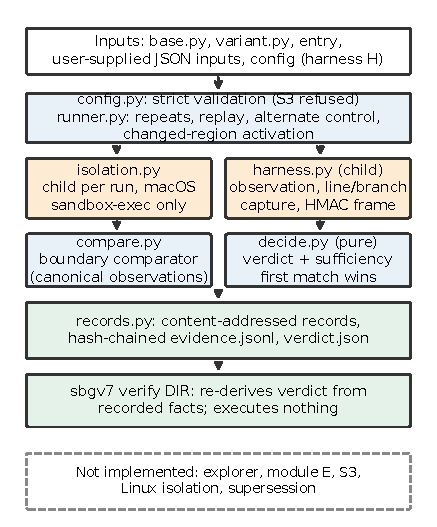
\includegraphics[width=0.92\columnwidth]{../../results/v7b_phase2_summary/figures/fig_p2_architecture.pdf}
\caption{V7-B modules and data flow (generated by \texttt{scripts/p2\_make\_paper\_figures.py}; no external diagram tool). Dashed box: specified but not implemented.}\label{fig:arch}
\end{figure}

For each input the runner executes each version $r_{det}=3$ times (early stop on disagreement); if the versions differ it performs $r_{replay}=5$ fresh replays per side and, if a controlled source was consulted, $k_{alt}=3$ alternate-control runs. Alternate runs virtualise seeded random, wall-clock functions based on \texttt{time.time}, and monotonic and performance counters, and seed \texttt{os.urandom} and \texttt{uuid4}; \texttt{datetime.now} and \texttt{secrets} are \emph{not} virtualised. The decision function then applies the verdict table of Section~\ref{sec:verdicts}.

\textbf{Implementation conformance status.} Against the 135 rules of the frozen specification the reconciled traceability matrix records 78 conforming, 30 partially conforming, 7 deviating, 14 not implemented, 2 unverifiable and 4 deferred to Phase 3 (78+30+7+14+2+4=135; \path{reports/phase2/PHASE2_TRACEABILITY_RECONCILIATION.md}). This is an implementation conformance status only. It says how much of a specification the code follows, not that the specification is right, that thresholds are calibrated, or that the system performs well. The unit tests executed with the E3 run were 286 passed and 1 skipped (\texttt{tests/v7} and \texttt{tests/v6}).

\textbf{Result channel.} The harness returns its result as one HMAC-authenticated frame on a dedicated pipe with a per-run key; a missing, duplicate, malformed or forged frame is a protocol violation that blocks both \DIV{} and \NDO{} (primary reason \texttt{unsafe\_program}). This is a local protocol-correctness fix, not a security boundary: the untrusted program shares the harness address space and can in principle recover the key.

\section{Evidence and Witness Model}\label{sec:evidence}
Every record carries an evidence class (observation, derived, inferred, proof) and an optional status in the specification. Runs and reproducibility checks are observations; the changed-region record and the witness difference are derived; the sufficiency record is derived and marked uncertain. Records are content-addressed and appended to a hash-chained JSONL log. The log holds an evidence package (configuration and $H$, harness digest, environment, policy, inputs, per-input rows with run ids, regions) so that \texttt{verify} can rebuild changed regions from the stored sources, re-derive each input outcome from the stored runs and re-run the decision function, requiring value, level, reasons and witness to match the recorded verdict. A trace function walks a verdict to its witness or sufficiency record, then to the runs and observations behind it. The run-set commitment inside the sufficiency record is a Merkle root; the log itself is a flat hash chain, not a Merkle tree.

\textbf{Integrity status (limited).} The chain is a plaintext, unkeyed SHA-256 chain with content-addressed ids. It detects accidental corruption and inconsistent edits. It is \emph{not tamper-proof}, and it is tamper-evident only in the limited sense above, not against a deliberate writer: anyone who can write the evidence directory can edit records, recompute every id and chain hash and rewrite \texttt{verdict.json} together with its \texttt{log\_head}, and \texttt{verify} will pass, because it checks verdict logic and chain consistency, not who wrote the facts. \texttt{verify} takes recorded observations, per-run status and sandbox capability states as given; it executes nothing. A trust anchor outside the writer's reach (a pinned \texttt{log\_head} or a signature) does not exist and is Phase 3 work. Experiment E7 exercised these properties (Section~\ref{sec:results}, Table~\ref{tab:e7}). The log is plaintext and contains source code, inputs and captured output, without redaction.

\section{Sufficiency}\label{sec:sufficiency}
Sufficiency is a conjunction of floors on separately reported factors; it is recorded, never scored as a probability.
\begin{itemize}
\item \textbf{S0}: a label for ``an S1 floor fails''; it appears only inside \INS.
\item \textbf{S1}: at least one deterministic-confirmed \texttt{same} input valid on both versions (not lossy and not degenerate); all changed units hit; no quarantined input that may hit a changed unit; no truncation, blind spot or tamper flag.
\item \textbf{S2}: S1 plus branch-direction coverage of changed regions of at least the floor (default 0.80) per version, every contributing input deterministic-confirmed, and no lossy-equal observation on return or side channels.
\item \textbf{S3}: specified (plateau, trace stability, second explorer) but \textbf{not implemented}: it is refused in configuration and never emitted. The S3 row of the risk--coverage table (Table~\ref{tab:riskcov}) therefore holds only witnessed divergences.
\end{itemize}
The 0.80 floor is an unvalidated default and no calibration was performed. Experiment E5 varied it (Section~\ref{sec:ablation}). Branch coverage counts conditional jumps, loop and send instructions only, with a conservative denominator. An independent review showed that S2 can be reached from two inputs, because levels do not depend on input count or diversity. S1 and S2 must therefore not be read as a quality grade or as ``80\% of changed branch directions validated as behaviourally safe'', and no evidence shows that they discriminate correct from incorrect verdicts. Sufficiency is also a contested proxy~\cite{inozemtseva2014coverage,just2014mut}.

\section{Verdict Generation}\label{sec:verdicts}
The first matching rule applies (Fig.~\ref{fig:verdictflow}): (1) identical sources give no verdict; (2) any confirmed-difference input gives \DIV; (3) any blocking condition gives \INS{} with the lowest-ranked code as primary reason and the others as secondary; (4) otherwise \NDO{} at the highest level whose floors hold. Blocking conditions include import or entry failure; unsupported signature or alignment failure; sandbox failure; unconfirmed or environment-sensitive candidate; unmodelled changed lines; a quarantined input; exactly one side limited; truncated capture; no usable input or unobservable (lossy) outcome; an unactivated changed unit; and an S1 floor failing. The reason-code enumeration is closed (18 codes); several codes are rarely or never produced (ambiguous entry, blind-spot dominance), so the \INS{} vocabulary is partly aspirational.

\begin{figure}[t]\centering
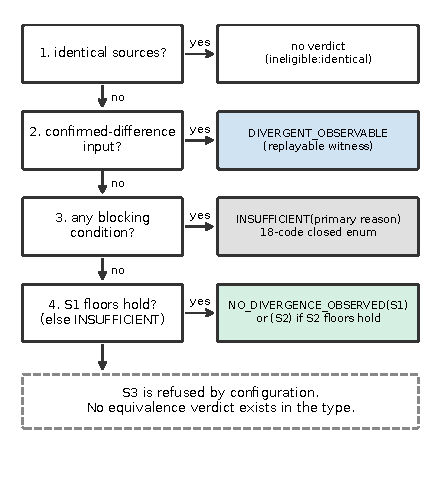
\includegraphics[width=0.92\columnwidth]{../../results/v7b_phase2_summary/figures/fig_p2_verdict_flow.pdf}
\caption{Verdict flow: first match wins; no equivalence verdict exists.}\label{fig:verdictflow}
\end{figure}

Equivalence cannot be emitted because the verdict type asserts a closed value set; this is a naming guarantee. Two rules of the Phase 2 engine matter for the results. First, an equality established on a lossy or degenerate canonical form does not count as the S1 input. Second, changed lines without executable code (for example a continuation line of a multi-line statement) are \texttt{unmodelled\_change}, a conservative blocker (rule A-U1); the rule is unrefined, because continuation lines of an executable statement are not mapped to the statement, and its refinement is an open design decision. A defect found earlier by independent review (a no-run input silently dropped, making \NDO{} reachable with an incomplete input) was fixed before Phase 2.

\section{Execution Isolation and Determinism}\label{sec:execution}
Each run is a fresh child process (\texttt{python -s -P -B}, an allowlisted environment, a private working directory), wrapped on macOS in \texttt{sandbox-exec} with a deny-network, write-confined profile; resource limits (CPU, file size, open files) are set in the child and a parent watchdog kills the process group. The platform was one Apple M4 Pro machine (macOS 26.7, arm64) with CPython 3.13.15. Memory limits rely on parent polling; address-space and process-count limits are not enforced on this platform; reads are not confined; a child that detaches into a new session could escape the group kill (untested); \texttt{sandbox-exec} is deprecated. Every record carries a flag that the isolation policy is below the specification minimum, which the specification classes as synthetic or benchmark-only grade. \textbf{Linux, Docker and OS-level isolation were not implemented, not tested and not validated. No claim of safe execution of untrusted code and no cross-platform claim is made.}

\textbf{Determinism controls.} Children run with \texttt{PYTHONHASHSEED=0}, \texttt{TZ=UTC}, \texttt{LC\_ALL=C.UTF-8} and single-threaded numerics. \textbf{Determinism is not complete.} The hash seed is fixed and never varied, so hash-order (set-iteration) sensitivity is untested and a fixed seed removes that variation by construction without showing it harmless; \texttt{datetime.now} is not virtualised, so wall-clock-dependent programs can still yield false witnesses; process ids, thread scheduling and addresses are not controlled; and witness identity is timing-dependent for inputs that sit near a resource limit (Section~\ref{sec:failure}). Experiment E2 (hash-order sensitivity) was deliberately not run.

\section{Methodology}\label{sec:method}
The study is a local, exploratory development analysis. V7-B and its baselines were shaped while seeing these data, no sealed or independent holdout exists, and the confirmatory gate K5 (at least 60 projects, at least 250 adjudicated divergent pairs, kappa of at least 0.7, clean leakage audit) was not attempted. The real-pair feasibility gate K1 (at least 100 runnable real pairs from at least 8 projects under validated Linux isolation) is neither triggered nor cleared; K1, K5 and all Phase 3 work are deferred. Under these conditions every inferential statement below is descriptive.

The protocols for E3--E7 and the hypothesis and decision rule for E1 were written and committed before the corresponding runs (\path{reports/phase2/E3_E7_PROTOCOLS.md}, \path{reports/phase2/LOCAL_EXPERIMENT_RERUN_MATRIX.md}); this pre-registration is internal and does not make the study confirmatory. Pipeline: run V7-B on the 321 pairs through its command-line interface (per-run limits of 2~s CPU and 5~s wall, four workers in E1, E3 and E4, sequential execution in E6); run the baselines on identical inputs; build one table of (pair, system) rows; analyse with a project-cluster bootstrap and project-level sign-flip tests (Section~\ref{sec:metrics}); verify every evidence directory with \texttt{verify} (E7). A pair is \emph{driven} when the engine supports its entry (top-level function); 9 pairs are not driven (eight class units and one unsupported entry policy) and count as failed or missing runs, that is abstention, in intention-to-treat accounting.

\section{Experimental Setup}\label{sec:setup}
All experiments ran on 2026-11-18 on one machine: Apple M4 Pro (14 cores, 48~GiB), macOS 26.7, arm64, CPython 3.13.15, \texttt{PYTHONHASHSEED=0} in every child. E1 ran at engine commit \texttt{a6afa639}; E3--E6 at commit \texttt{ee4749bc} (the per-run \texttt{RUN\_RECORD.md} files are authoritative). Table~\ref{tab:experiments} summarises the experiments; \texttt{E2} (hash-order sensitivity) was deliberately not run.

\begin{table}[t]\centering\scriptsize\setlength{\tabcolsep}{3pt}
\caption{Phase 2 experiments (all local, exploratory, non-pristine data). Raw evidence archives are outside git; compact outputs are in \path{results/v7b_phase2_summary/}.}\label{tab:experiments}
\resizebox{\linewidth}{!}{%
\begin{tabular}{lp{0.42\linewidth}p{0.3\linewidth}}
\hline
Exp. & Objective and design & Data and systems \\
\hline
E1 & K2 re-measurement: quarantined (self-inconsistent) inputs not higher after the hash-seed and environment fix; old engine versus current engine & 312 driven pairs; two runs; 102 pairs re-run \\
E3 & Detection, false assurance, abstention against baselines; project-cluster bootstrap, sign-flip, McNemar, Holm & 258 labelled pairs; V7-B, B1, B1+rep, B3, B4 \\
E4 & Component ablations V1--V5 (config deltas) & 321 pairs; five variants \\
E5 & S2 branch-coverage floor 0.6, 0.8, 0.9 & 321 pairs; three floors \\
E6 & Runtime cost, fresh process per job, 5 repetitions, two runs & fixed 40-pair subset; V7-B, B1, B1+rep \\
E7 & \texttt{verify} on every evidence directory; corruption suite & 828 directories; 42 corruption cases \\
\hline
\end{tabular}}
\end{table}

\textbf{Protocol deviations (disclosed).} The first E3 attempt through the full evaluation script was killed after 77 CPU-minutes in an unrelated legacy test stage, and a second aborted at a documentation-wording guard; the reported E3 run replaces that stage by \texttt{pytest tests/v7 tests/v6} (286 passed, 1 skipped) and runs all other stages as in the full script; failed attempts produced no data. E6 was flagged by the pre-registered load rule, repeated once and both runs are reported; the machine was on battery power. The E3 baselines-stage wall time (20,880~s, apparently a machine suspend) is not used. E1's verify log column recorded the pipeline exit status; the \texttt{verified} field is the authority, and E7 re-verified with real exit codes.

\section{Datasets}\label{sec:datasets}
All 321 pairs are exposed or non-pristine: QuixBugs and BugsInPy are widely used benchmarks and were used in earlier evaluations of this programme, the synthetic pairs were scored by earlier-generation systems, and V7-B was shaped on them. There is no independent holdout and benchmark exposure cannot be excluded. They are development data, not evidence of field performance. The arms are (Table~\ref{tab:datasets}):
\begin{itemize}
\item \textbf{QuixBugs buggy/fixed} (31 pairs): inputs from the benchmark's declared test cases, outputs unused. Truth: divergent for the 29 pairs whose declared tests fail on the buggy and pass on the fixed version (a test-replay oracle independent of V7-B and the baselines); two are unlabelled. QuixBugs counts as one project.
\item \textbf{QuixBugs semantics-preserving negatives} (85): the fixed version against a generator-made semantics-preserving variant; label ``no observed difference''; one suspect.
\item \textbf{Synthetic changed} (78) and \textbf{synthetic equivalent} (72): generator labels; ``equivalent'' means equivalent under a looser equality than the V7-B boundary, so a witnessed pair may be a label artefact. Divergence in ``changed'' pairs may lie outside the sampled inputs.
\item \textbf{BugsInPy units} (55): real fixes, extracted single-file functions, run on synthetic battery inputs rather than project tests; nine class units are not driven. No defensible truth label exists, so all are excluded from primary denominators.
\end{itemize}
Six suspect labels are tagged and excluded but never relabelled. The primary denominators are 106 divergent-labelled and 152 no-difference-labelled pairs (258); 57 unlabelled pairs are excluded. The divergent pairs span 78 project clusters and the no-difference pairs 69; the largest cluster has 29 pairs (QuixBugs). Synthetic ``projects'' are generator base programs. No real independent project-level run exists.
\begin{table}[t]\centering\scriptsize\setlength{\tabcolsep}{3pt}
\caption{The 321 development pairs by arm and truth class (V7-B rows; all data non-pristine). Primary denominators: divergent (div.) and no-observed-difference (no-diff.) labels (258 pairs); suspect and unlabelled pairs are excluded. Source: \path{results/v7b_phase2_summary/p2_e3_20261118_092700/processed/dev_pairs_per_system.csv}.}\label{tab:datasets}
\resizebox{\linewidth}{!}{%
\begin{tabular}{lrrrrrl}
\hline
Arm & Pairs & Div. & No-diff. & Suspect & Unlab. & Truth rule \\
\hline
bugsinpy\_units & 55 & 0 & 0 & 0 & 55 & real fixes; no defensible label \\
quixbugs\_buggy\_fixed & 31 & 29 & 0 & 0 & 2 & declared tests fail on buggy, pass on fixed \\
quixbugs\_sp\_negatives & 85 & 0 & 84 & 1 & 0 & generator: semantics-preserving variant \\
synthetic\_equivalent & 72 & 0 & 68 & 4 & 0 & generator label: equivalent (looser equality) \\
synthetic\_changed & 78 & 77 & 0 & 1 & 0 & generator label: changed \\
total & 321 & 106 & 152 & 6 & 57 &  \\
\hline
\end{tabular}}
\end{table}


\section{Baselines}\label{sec:baselines}
Table~\ref{tab:baselines} lists the baselines. B1, B1+rep and B3 share V7-B's runner, inputs, comparator and CPU-budget unit. B1+rep adds exactly V7-B's repetition counts and is the null model for V7-B without its sufficiency gate and control alternation. Baselines never abstain, treat a missing entry or one-sided limit as a difference, and have no sufficiency level. B4's threshold is fitted on development material. Only B1, B1+rep, B3 and B4 enter the analysed tables.

\textbf{Published tools not compared.} Shadow symbolic execution, DiffKemp, Mokav, Testora, DiffTestGen, Cleverest, Prefactory, PatchGuru, ORION, SemaDiff and other LLM differential-testing tools, AFL, libFuzzer, Atheris and property-based generators (B3 is only a minimal analogue), differential unit testing, dynamic impact analysis, regression-verification provers, flaky-test tools and LLM equivalence judges were not implemented and not run. No empirical claim is made relative to any of them; the numbers reported by their authors are not comparable with ours.
\begin{table*}[t]
\centering\scriptsize
\caption{Baselines (from \path{research/evaluation/BASELINE_IMPLEMENTATION_AND_FAIRNESS.md}). B1--B3 share the runner, inputs, comparator and CPU budget unit with V7-B; baselines do not abstain.}
\label{tab:baselines}
\begin{tabular}{p{0.07\textwidth}p{0.4\textwidth}p{0.4\textwidth}}
\hline
ID & What it does & Status and caveat \\
\hline
B1 & same-input differential execution, one run per side, no repeats or sufficiency check & implemented; the same-budget reference for all paired comparisons; renamed-entry pairs count as differences \\
B1+rep & B1 plus $r_{det}=3$ and $r_{replay}=5$ repeats; no sufficiency gate, no control alternation & implemented and verified; the null model for V7-B minus sufficiency \\
B2 & declared-test replay (pass/fail per version) & QuixBugs only; uses expected outputs V7-B does not; not part of Phase 2 analysis \\
B3 & minimal coverage-guided mutation of arguments on top of B1 & implemented minimally; NOT a stand-in for AFL, libFuzzer or Hypothesis \\
B4 & edit-size heuristic with a threshold tuned on development data & no usable signal on these pairs \\
B5 & lookup of earlier-system (V6) scores from frozen artefacts & incomplete, not input- or budget-matched; not part of Phase 2 analysis \\
Published tools & Shadow SE, DiffKemp, Mokav, Testora, DiffTestGen, Cleverest, Prefactory, AFL-class fuzzers, regression-verification provers, flaky-test tools, LLM equivalence judges & NOT IMPLEMENTED; NOT COMPARED \\
\hline
\end{tabular}
\end{table*}


\section{Metrics and Statistical Methods}\label{sec:metrics}
Per system: \emph{detection} = P(\DIV{} $\mid$ divergent label); \emph{false assurance} = P(\NDO{} $\mid$ divergent label); \emph{abstention} = P(\INS{} or failed run) over the primary denominator of 258; \emph{false alarm} = P(\DIV{} $\mid$ no-difference label); \emph{risk--coverage} with coverage = decided/eligible and risk = errors/decided, where errors are \NDO{} on a divergent label or \DIV{} on a no-difference label. Detection and false assurance are the primary family; the rest are secondary. Failed or missing runs count as abstention (intention-to-treat). Baseline outputs map DIVERGE to \DIV{} and NO\_DIFF to \NDO{}. Labels are generator labels or test-oracle truth and are not adjudicated, so ``false assurance'' means ``no difference reported on a pair labelled divergent'', not a verified miss.

\textbf{Inference.} The inference unit is the project (78 clusters among divergent pairs, 69 among no-difference pairs). Rates are ratios with a project-cluster percentile bootstrap (95\%, $B=10000$, seed 42). Paired comparisons use a project-level sign-flip test, an exact McNemar test at pair level as a sensitivity check, and Holm correction within the pre-registered family (4 comparisons $\times$ 2 primary outcomes). The effect-of-interest rule requires the false-assurance improvement to be at least +10 percentage points with a lower confidence bound above +10. With few independent projects and one dominant cluster, percentile bootstrap intervals can undercover; all $p$-values are descriptive because pairs cluster by project, some labels are synthetic and the data are non-pristine. Power is a design-property simulation, not post-hoc power at the observed effect.

\textbf{Attribution of the false-assurance reduction.} For the pairs that B1 wrongly passes, we cross-tabulate the V7-B verdict. A reduction is ``abstention'' when the recovered pairs become \INS{} rather than \DIV{}. We also report a derived, not executed, gate counterfactual that relabels \INS{} verdicts as \NDO{} (Table~\ref{tab:gate}).

Section~\ref{sec:stats} classifies each finding as supported, descriptive, exploratory, inconclusive or unsupported. Table~\ref{tab:notevaluated} lists what is not evaluated.
\begin{table*}[t]
\centering\scriptsize
\caption{NOT EVALUATED register (Phase 2; sources: \path{reports/phase2/PHASE2_CONSOLIDATED_EXPERIMENTAL_ANALYSIS.md}, section 10, and \path{reports/phase2/K1_K5_READINESS_AND_DECISION.md}).}
\label{tab:notevaluated}
\begin{tabular}{p{0.27\textwidth}p{0.14\textwidth}p{0.5\textwidth}}
\hline
Item & Status & Reason \\
\hline
Confirmatory family and independent generalisation (RQ5) & NOT EVALUATED & no sealed holdout; data non-pristine; K5 not attempted; no independent real project-level run \\
Superiority over any like-for-like comparator; matched-coverage false assurance & NOT EVALUATED & only raw counts; no matched-coverage computation \\
Truth for BugsInPy units, two QuixBugs pairs, six suspect labels & NOT EVALUATED & no defensible label; never relabelled \\
K1 (real-pair feasibility) and K2 under validated isolation & DEFERRED (Phase 3) & neither triggered nor cleared; needs Linux/Docker isolation \\
Linux, Docker and OS-level isolation & NOT VALIDATED & macOS \texttt{sandbox-exec} only; policy flagged below minimum \\
Tamper evidence against a deliberate writer & NOT PROVIDED & unkeyed hash chain; no trust anchor \\
Complete determinism: hash-order sensitivity (E2), \texttt{datetime.now} & NOT EVALUATED & hash seed fixed and never varied; clock not virtualised \\
Published tools (Shadow SE, DiffKemp, Testora, Cleverest, Prefactory, etc.) & NOT COMPARED & not implemented or run; no claim relative to them \\
S3, explorer, module E, declared renames, generator entries & NOT IMPLEMENTED & contribute to \texttt{unsupported\_signature} and abstention \\
Component value of replay, control alternation and thresholds & NOT SHOWN & ablations change no verdict (data have almost no nondeterminism) \\
Calibration of the 0.80 branch floor and repeat counts & NOT EVALUATED & defaults are unvalidated; E5 shows only that the floor relabels S1/S2 \\
Refinement of \texttt{unmodelled\_change} & OPEN & rule is conservative and unrefined (UD-2) \\
Cross-language, cross-platform & NOT SUPPORTED & Python on macOS only \\
\hline
\end{tabular}
\end{table*}


\section{Results (Exploratory)}\label{sec:results}
\emph{All numbers are descriptive, from the 321 non-pristine development pairs, local macOS runs on 2026-11-18. They are not evidence of performance in the field. Each table and figure names its source under \path{results/v7b_phase2_summary/}.}

\subsection{E1: determinism re-measurement (K2, weak)}
The pre-registered hypothesis was that the quarantined rate does not rise after the corrected child environment and hash-seed configuration. Of 312 driven pairs, 1 has at least one quarantined input under the current engine versus 2 under the earlier engine (1 versus 3 of 3,044 inputs); the new-only versus old-only discordant pairs are 0 versus 1 (one-sided exact $p=1.0$). By the pre-registered rule the hypothesis is \emph{supported, weakly}: the counts are tiny, pairs cluster by project, and the comparison is confounded, because the old child profile (\texttt{-I}) ignored \texttt{PYTHONHASHSEED} and the two engines also differ in other fixes. It is an old-engine versus current-engine comparison, not a seed effect, and it is not evidence of determinism. The pair that left quarantine (\texttt{graph\_center\_finder}) is consistent with set-order dependence, which is untested; one pair (\texttt{black\_\_21\_\_black\_py\_\_dump\_to\_file}) is quarantined in both runs. Re-running 102 pairs gave identical verdicts, levels, reasons and witness ids in 102 of 102 cases, and all 414 evidence directories verified.

E1 also exposed a change in the verdict distribution (Fig.~\ref{fig:verdictdist}): 63 of 312 verdicts changed and the number of \DIV{} is unchanged at 84. The principal transition is 37 pairs from \NDO{}/S2 to \INS{}(\texttt{unmodelled\_change}), plus 14 from \texttt{changed\_region\_not\_activated} to \texttt{unmodelled\_change}; in total 54 pairs now abstain with \texttt{unmodelled\_change} (27 QuixBugs negatives, 17 synthetic, 10 BugsInPy). Of these, three evidence packages were inspected: changed lines lay inside multi-line statements (a regex string literal, a list-literal element) that the earlier engine ignored; the other transitions were not individually inspected.
\begin{figure}[t]\centering
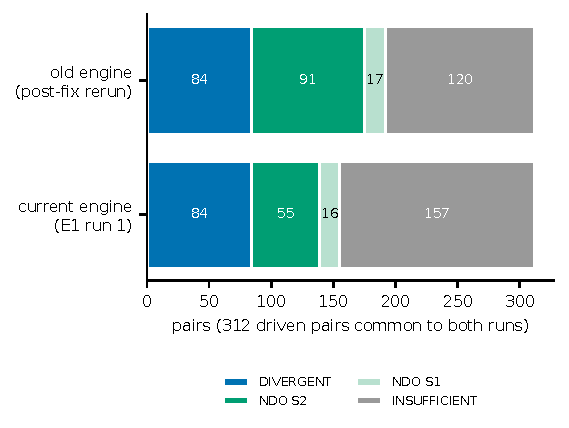
\includegraphics[width=\columnwidth]{../../results/v7b_phase2_summary/figures/fig_p2_verdict_dist.pdf}
\caption{V7-B verdict distribution on the 312 driven pairs: earlier engine (post-fix rerun) versus current engine (E1 run 1). Source: \path{results/v7b_phase2_summary/p2_e1_20261118_074906/e1_analysis.json}.}\label{fig:verdictdist}
\end{figure}

\subsection{E3: detection, false assurance and abstention}
Table~\ref{tab:datasets} gives the data and Table~\ref{tab:byarm} the V7-B verdict per arm (84 \DIV{}, 157 \INS{}, 16 \NDO{}/S1, 55 \NDO{}/S2, 9 not driven). Table~\ref{tab:metrics} and Fig.~\ref{fig:metrics} give the system metrics on the 258 labelled pairs. V7-B returns \NDO{} on 13 of 106 divergent-labelled pairs (0.123) against 24 of 106 for B1 (0.226) and B1+rep (identical; 0 discordant pairs), and detects 75 of 106 (0.708) against 82 of 106 (0.774). V7-B abstains on 122 of 258 pairs (0.473; 18 divergent-labelled and 104 no-difference-labelled) and raises no false alarm on the 152 no-difference-labelled pairs, whereas B1 reports a difference on 46 of 152 (0.303). The edit-size heuristic B4 has no usable signal (1 of 106 detected).
\begin{table}[t]\centering\scriptsize\setlength{\tabcolsep}{3pt}
\caption{E3 system metrics on the 258 labelled pairs (106 divergent, 152 no-difference); 95\% project-cluster bootstrap CI ($B=10000$, seed 42). Exploratory; non-pristine data. Abstention for V7-B counts INSUFFICIENT on both truth classes (122 = 18 + 104). Source: \path{results/v7b_phase2_summary/p2_e3_20261118_092700/statistics/system_metrics.csv}.}\label{tab:metrics}
\resizebox{\linewidth}{!}{%
\begin{tabular}{lllll}
\hline
System & False assurance & Detection & Abstention & False alarm \\
\hline
B1 & 24/106 = 0.226 [0.119, 0.392] & 82/106 = 0.774 [0.609, 0.881] & 0/258 & 46/152 = 0.303 \\
B1+rep & 24/106 = 0.226 [0.120, 0.390] & 82/106 = 0.774 [0.610, 0.880] & 0/258 & 46/152 = 0.303 \\
B3 & 20/106 = 0.189 [0.097, 0.337] & 86/106 = 0.811 [0.662, 0.904] & 0/258 & 47/152 = 0.309 \\
B4 & 105/106 = 0.991 [0.981, 1.000] & 1/106 = 0.009 [0.000, 0.019] & 0/258 & 1/152 = 0.007 \\
V7-B & 13/106 = 0.123 [0.054, 0.236] & 75/106 = 0.708 [0.545, 0.816] & 122/258 = 0.473 [0.353, 0.524] & 0/152 = 0.000 \\
\hline
\end{tabular}}
\end{table}

\begin{figure*}[t]\centering
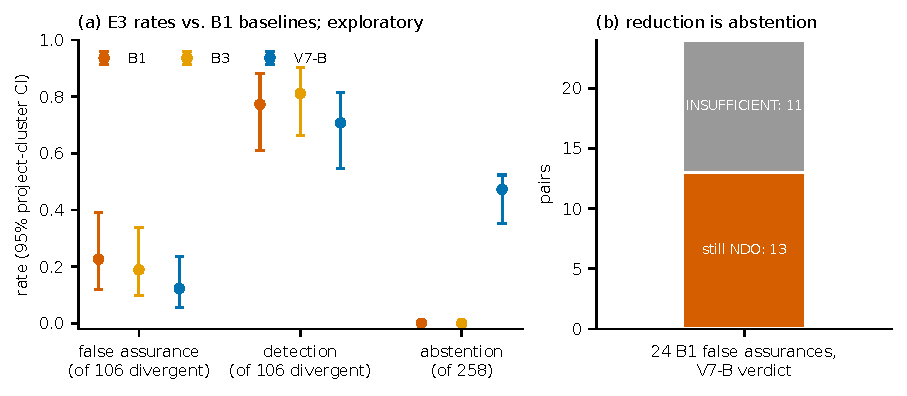
\includegraphics[width=0.85\textwidth]{../../results/v7b_phase2_summary/figures/fig_p2_metrics_vs_b1.pdf}
\caption{(a) Rates with 95\% project-cluster intervals for B1, B3 and V7-B. (b) The verdict of V7-B on the 24 pairs that B1 wrongly passes. Source: \path{results/v7b_phase2_summary/p2_e3_20261118_092700/statistics/system_metrics.csv} and \path{.../processed/dev_pairs_per_system.csv}.}\label{fig:metrics}
\end{figure*}

\textbf{Paired comparison.} Table~\ref{tab:paired} compares V7-B with B1 on the 106 divergent pairs. The false-assurance difference is $-10.4$ points (95\% CI $[-20.5,-4.3]$; 0 V7-B-only versus 11 B1-only discordant pairs; sign-flip $p=0.0010$, exact McNemar $p=0.0010$, Holm $p=0.0059$). \textbf{The +10 point rule is not met} (the improvement's lower confidence bound is 4.3 points), so the defensible wording is ``reduced by about 10 points, not shown to reach 10''. Detection is $-6.6$ points ($[-11.5,-2.6]$; 0 versus 7; sign-flip $p=0.031$; Holm $p=0.156$): a possible loss, not significant after correction and not an established harm. B3 versus B1 is not significant (sign-flip $p=0.125$, Holm 0.5). Neither the intervals nor the $p$-values license a generalisation (Section~\ref{sec:stats}).
\begin{table}[t]\centering\scriptsize\setlength{\tabcolsep}{3pt}
\caption{Paired comparisons against B1 (difference in rate, test minus reference, with 95\% project-cluster CI; test-only/ref-only discordant pairs; project-level sign-flip, exact McNemar, Holm over 4 comparisons $\times$ 2 primary outcomes). Descriptive: pairs cluster by project, data are non-pristine. The +10pp rule is not met in any row. Source: \path{results/v7b_phase2_summary/p2_e3_20261118_092700/statistics/paired_comparisons.csv}.}\label{tab:paired}
\resizebox{\linewidth}{!}{%
\begin{tabular}{llrrrrrr}
\hline
Comparison & Outcome & Diff. [CI] & b/c & Sign-flip p & McNemar p & Holm p & +10pp \\
\hline
V7-B vs B1 & false assurance & -0.104 [-0.205, -0.043] & 0/11 & 0.0010 & 0.0010 & 0.0059 & no \\
V7-B vs B1 & detection & -0.066 [-0.115, -0.026] & 0/7 & 0.0312 & 0.0156 & 0.1562 & no \\
V7-B vs B1 & abstention & +0.473 [+0.354, +0.523] & 122/0 & <1e-4 & <1e-4 & 0.0003 & no \\
V7-B vs B1 & false alarm & -0.303 [-0.352, -0.145] & 0/46 & <1e-4 & <1e-4 & 0.0002 & no \\
B3 vs B1 & false assurance & -0.038 [-0.090, -0.007] & 0/4 & 0.1250 & 0.1250 & 0.5000 & no \\
B3 vs B1 & detection & +0.038 [+0.007, +0.090] & 4/0 & 0.1250 & 0.1250 & 0.5000 & no \\
B1+rep vs B1 & detection & +0.000 [+0.000, +0.000] & 0/0 & 1.0000 & 1.0000 & 1.0000 & no \\
\hline
\end{tabular}}
\end{table}


\textbf{The reduction is entirely abstention.} Of the 24 divergent pairs that B1 (and B1+rep) wrongly pass, V7-B returns \INS{} for 11 and \NDO{} for 13 and detects none of them (Fig.~\ref{fig:metrics}b); the pre-registered attribution statistic is 11 of 11 recovered cases being \INS{} (the cluster-bootstrap interval is degenerate at $[1,1]$ because all 11 are \INS{}, and with $n=11$ it is not a precise estimate). On the 88 divergent pairs where V7-B does not abstain, V7-B detects 75 and misses 13, and B1 detects the same 75 and misses the same 13. V7-B's advantage on false assurance is therefore calibrated abstention, not extra detection. The derived, not executed, gate counterfactual (Table~\ref{tab:gate}) shows the same: relabelling every \INS{} as \NDO{} raises false assurance from 13 to 31 of 106 (0.293), and relabelling only the gate-attributable reasons gives 24 of 106 (0.226), equal to B1.
\begin{table}[t]\centering\scriptsize\setlength{\tabcolsep}{3pt}
\caption{Derived (not executed) gate counterfactual on the E3 verdicts. Source: \path{results/v7b_phase2_summary/p2_consolidated_20261118_190644/consolidated.json}, key \texttt{gate\_counterfactual\_E3}.}\label{tab:gate}
\resizebox{\linewidth}{!}{%
\begin{tabular}{lrrr}
\hline
Variant & False assurance & Rate & Abstained \\
\hline
actual V7-B & 13/106 & 0.123 & 122 \\
all INSUFFICIENT relabelled NDO & 31/106 & 0.292 & 0 \\
only gate-attributable reasons relabelled & 24/106 & 0.226 & 96 \\
\hline
\end{tabular}}
\end{table}


\textbf{Risk--coverage.} Table~\ref{tab:riskcov} and Fig.~\ref{fig:riskcov} show that V7-B decides 136 of 258 pairs (coverage 0.527; the 0.096 figure is 13/136 and mixes 75 detections with 61 \NDO{} verdicts, so it is not the error rate of \NDO{}: 13 of 61 \NDO{} verdicts are wrong versus 24 of 130 for B1) at any level, and 120 of 258 (coverage 0.465, risk 0.067) when \NDO{} requires S2; B1 decides all pairs at risk 0.271. The S3 row (coverage 0.291, 75 decided, risk 0) contains only witnessed divergences, because S3 is refused by configuration. The curve is descriptive: risk is against generator labels, baselines have no sufficiency level, and matched-coverage superiority was not computed.
\begin{table}[t]\centering\scriptsize\setlength{\tabcolsep}{3pt}
\caption{Risk--coverage (decided verdicts only; risk = errors/decided against generator or test-oracle labels). The V7-B S3 row contains only witnessed divergences because S3 is refused by configuration and no NO\_DIVERGENCE\_OBSERVED is issued at that level. Source: \path{results/v7b_phase2_summary/p2_e3_20261118_092700/statistics/risk_coverage.csv}.}\label{tab:riskcov}
\resizebox{\linewidth}{!}{%
\begin{tabular}{llrrr}
\hline
System & Min. level for NDO & Coverage & Risk [CI] & Decided \\
\hline
B1 & none & 1.000 & 0.271 [0.210, 0.331] & 258/258 \\
V7-B & none & 0.527 & 0.096 [0.038, 0.212] & 136/258 \\
V7-B & S1 & 0.527 & 0.096 [0.039, 0.210] & 136/258 \\
V7-B & S2 & 0.465 & 0.067 [0.023, 0.167] & 120/258 \\
V7-B & S3 & 0.291 & 0.000 [0.000, 0.000] & 75/258 \\
\hline
\end{tabular}}
\end{table}

\begin{figure}[t]\centering
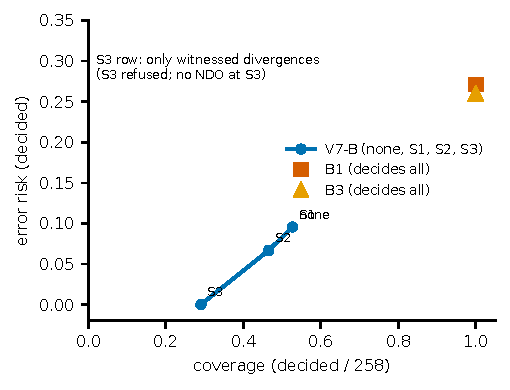
\includegraphics[width=\columnwidth]{../../results/v7b_phase2_summary/figures/fig_p2_risk_coverage.pdf}
\caption{Coverage versus error risk (descriptive; generator and test-oracle labels). Source: \path{results/v7b_phase2_summary/p2_e3_20261118_092700/statistics/risk_coverage.csv}.}\label{fig:riskcov}
\end{figure}

\textbf{Change relative to the earlier post-fix run.} Detection (0.708) and false assurance (0.123) are unchanged and baselines are identical, but abstention rose from 0.360 to 0.473 because 54 pairs now return \INS{}(\texttt{unmodelled\_change}) (Table~\ref{tab:reasons}). This is the conservative rule A-U1, which is unrefined; part of the increase may be noise of that rule, and only three of the affected pairs were inspected. It is not shown that the shift reduced false assurance.
\begin{table}[t]\centering\scriptsize\setlength{\tabcolsep}{3pt}
\caption{Primary reason of the INSUFFICIENT verdicts in the E3 run (312 driven pairs; 9 pairs are not driven). Source: \path{results/v7b_phase2_summary/p2_e3_20261118_092700/processed/k1_spike_per_pair.jsonl}.}\label{tab:reasons}
\resizebox{\linewidth}{!}{%
\begin{tabular}{lrl}
\hline
Primary reason & Pairs & Meaning \\
\hline
unmodelled\_change & 54 & changed lines without executable code (rule A-U1) \\
unsupported\_signature & 49 & renamed entry or unsupported signature \\
changed\_region\_not\_activated & 40 & no input reached the changed lines \\
unobservable\_outcome & 8 & lossy or degenerate observation \\
resource\_limit & 4 & limit hit on a side or both \\
nondeterministic & 1 & a version is not self-consistent \\
import\_error & 1 & import or entry failure \\
total & 157 &  \\
\hline
\end{tabular}}
\end{table}

\begin{table}[t]\centering\scriptsize\setlength{\tabcolsep}{3pt}
\caption{V7-B verdict per arm, E3 run (321 pairs). Source: \path{results/v7b_phase2_summary/p2_e3_20261118_092700/processed/dev_pairs_per_system.csv}.}\label{tab:byarm}
\resizebox{\linewidth}{!}{%
\begin{tabular}{lrrrrr}
\hline
Arm & DIV & INSUF. & NDO S1 & NDO S2 & Not driven \\
\hline
bugsinpy\_units & 6 & 32 & 0 & 8 & 9 \\
quixbugs\_buggy\_fixed & 27 & 4 & 0 & 0 & 0 \\
quixbugs\_sp\_negatives & 1 & 60 & 3 & 21 & 0 \\
synthetic\_equivalent & 1 & 45 & 8 & 18 & 0 \\
synthetic\_changed & 49 & 16 & 5 & 8 & 0 \\
total & 84 & 157 & 16 & 55 & 9 \\
\hline
\end{tabular}}
\end{table}


\subsection{E4--E6: ablation, S2 floor and runtime}
The results of E4 and E5 are in Section~\ref{sec:ablation} and those of E6 in Section~\ref{sec:runtime}.

\subsection{E7: verification and corruption suite}
\texttt{python -m sbgv7 verify} returned exit 0 for all 828 evidence directories (E3 and E1, run 1 and run 2), covering \DIV{}, \NDO{}/S1, \NDO{}/S2 and \INS{} with every reason code produced. On copies, the corruption suite behaved as pre-registered in 42 of 42 runs (Table~\ref{tab:e7}): a flipped byte, truncation, a deleted record, a missing package, a broken chain, an edited \texttt{verdict.json}, a deleted log (exit 2) and a simulated size-cap omission (exit 4) are detected, and a modification without re-chaining is detected. The documented limitations behave as predicted and are \emph{not} detected: a writer who edits unverified fields (run timings, run status or detail) and recomputes the chain and \texttt{log\_head} produces a log that verifies, and a deleted \texttt{verdict.json} is not detected. \texttt{verify} recomputes recorded facts and executes nothing, so it cannot detect a lie in a recorded observation. 828 of 828 verified is therefore consistency of the records, not validation of the system and not tamper-proofing.
\begin{table}[t]\centering\scriptsize\setlength{\tabcolsep}{3pt}
\caption{E7 corruption suite: 14 corruption cases applied to copies of three evidence directories each (one per verdict class), 42 runs. Exit codes of \texttt{verify}: 0 verified, 1 mismatch, 2 unreadable or missing, 4 evidence omitted by size cap. ``As expected'' means as pre-registered; cases ending with exit 0 are documented limitations that the check does not detect. Source: \path{results/v7b_phase2_summary/p2_e7_20261118_190612/corruption_results.json}.}\label{tab:e7}
\resizebox{\linewidth}{!}{%
\begin{tabular}{lrrrl}
\hline
Case & Runs & Exit code & As expected & Outcome \\
\hline
flip\_byte\_in\_record & 3 & 1 & yes & detected \\
truncate\_drop\_last\_record & 3 & 1 & yes & detected \\
truncate\_mid\_line & 3 & 1 & yes & detected \\
delete\_middle\_record & 3 & 1 & yes & detected \\
remove\_package\_rechained & 3 & 1 & yes & detected \\
break\_chain\_prev & 3 & 1 & yes & detected \\
verdict\_json\_changed & 3 & 1 & yes & detected \\
verdict\_json\_log\_head\_changed & 3 & 1 & yes & detected \\
evidence\_missing & 3 & 2 & yes & detected \\
source\_omitted\_rechained & 3 & 4 & yes & detected \\
forge\_meta\_timing\_rechained & 3 & 0 & yes & NOT detected (documented limit) \\
forge\_run\_status\_rechained & 3 & 0 & yes & NOT detected (documented limit) \\
forge\_without\_rechain & 3 & 1 & yes & detected \\
delete\_verdict\_json & 3 & 0 & yes & NOT detected (documented limit) \\
\hline
\end{tabular}}
\end{table}


\section{Statistical Analysis: What Is Supported}\label{sec:stats}
Table~\ref{tab:status} classifies each finding. ``Supported'' means supported descriptively on these exploratory data after the pre-registered correction; it does not mean confirmed. Multiple-comparison control is Holm within each pre-registered family (E3: 8 tests; E4 and E5 their own families); no $p$-value is a claim of significance across the campaign. The design-property power simulation gives at most 0.267 power for a +5 point difference at the observed discordance and no reachable power for +10 points (\path{statistics/power_actual.json}); the study could not have supported a confirmatory claim.

\begin{table}[t]\centering\scriptsize\setlength{\tabcolsep}{3pt}
\caption{Statistical status of the Phase 2 findings (source: \path{reports/phase2/PHASE2_CONSOLIDATED_EXPERIMENTAL_ANALYSIS.md}, section 8).}\label{tab:status}
\resizebox{\linewidth}{!}{%
\begin{tabular}{lp{0.65\linewidth}}
\hline
Status & Finding \\
\hline
Supported (descriptive, clustered, exploratory) & V7-B has lower false assurance than B1 (13/106 versus 24/106; Holm $p=0.0059$; +10 point rule not met) (the false-assurance reduction is fully attributable to abstention (11 of 11) and to B1 lacking a sufficiency gate; abstention is selective, 11 of 24 B1 false assurances versus 7 of 82 B1 detections became \\INSUFFICIENT, but precision of \\NDO{} verdicts is not better: 13/61 wrong versus 24/130 for B1)\\
Descriptive & detection 75/106 versus 82/106 (a possible loss: CI $[-11.5,-2.6]$ excludes zero, Holm $p=0.156$); false alarm 0/152 versus 46/152 (an artefact: all 46 B1 false alarms are renamed-entry pairs that B1 treats as differences, V7-B abstains on all 48 such pairs, and the pre-declared exclusion sensitivity was not run); abstention 122/258; runtime ratios; E5 stability; E4 invariance \\
Exploratory & attribution to specific mechanisms (\texttt{unmodelled\_change}, set-order dependence) \\
Inconclusive & any effect of the hash-seed change on determinism (1 versus 2 pairs); component value (no nondeterminism in the data) \\
Unsupported & independent generalisation; superiority beyond these 258 non-pristine pairs; comparison with published tools; OS isolation; tamper-proof evidence; complete determinism; hash-order robustness \\
\hline
\end{tabular}}
\end{table}

\section{Ablation and Sensitivity}\label{sec:ablation}
\textbf{E4: component ablations.} Five variants were run on all 321 pairs through configuration deltas (Table~\ref{tab:e4}): V1 $r_{det}=1$, V2 $r_{replay}=1$, V3 $k_{alt}=0$, V4 all three, V5 the fd-1 stdout fold off. \textbf{No variant changes the verdict value or level on any of the 321 pairs}; detection, false assurance, abstention and false alarm are identical and all paired $p$-values are 1.0 (no discordant pairs). The only observable difference is one reason code: \texttt{black\_\_21\_\_black\_py\_\_dump\_to\_file} moves from \texttt{nondeterministic} to \texttt{flaky\_witness} under V1 and V4 (both \INS{}). Witness ids change under V2--V4 because the replay set is part of the witness (84 pairs). V0 equals E3 on 320 of 321 strict keys; the exception is explained in Section~\ref{sec:failure}.
\begin{table}[t]\centering\scriptsize\setlength{\tabcolsep}{3pt}
\caption{E4 ablations on the 321 pairs (verdict counts; flips = pairs whose verdict value or level differs from V0). CPU is the summed per-pair CPU of the run (concurrency 4, load-sensitive). Only a reason code changes (one pair, V1 and V4). Source: \path{results/v7b_phase2_summary/p2_consolidated_20261118_190644/consolidated.json}, key \texttt{E4}.}\label{tab:e4}
\resizebox{\linewidth}{!}{%
\begin{tabular}{llrrrrr}
\hline
Variant & Change & DIV & INSUF. & NDO & Flips vs V0 & CPU s (sum) \\
\hline
V0 & default & 84 & 157 & 71 & -- & 546.8 \\
V1 & $r_{det}=1$ & 84 & 157 & 71 & 0 & 271.6 \\
V2 & $r_{replay}=1$ & 84 & 157 & 71 & 0 & 521.4 \\
V3 & $k_{alt}=0$ & 84 & 157 & 71 & 0 & 512.5 \\
V4 & V1+V2+V3 & 84 & 157 & 71 & 0 & 225.1 \\
V5 & FOLD\_FD1=False & 84 & 157 & 71 & 0 & 520.1 \\
\hline
\end{tabular}}
\end{table}

\textbf{Interpretation limit.} The dataset contains almost no intermittent or control-sensitive behaviour (E1: 1 of 312 pairs quarantined), so the confirmation machinery has nothing to filter. The experiment can show a cost (V4 uses about 65\% fewer runs, 4,746 versus 13,764 run records, for the same verdicts here) but \textbf{it cannot show the value of the components, and component importance must not be inferred}. The B1 versus B1+rep result (identical on all primary outcomes) points the same way and is equally uninformative about data containing real flakiness. Hash-order sensitivity is untested.

\textbf{E5: S2 branch-coverage floor.} The floor was run at 0.6, 0.8 (default) and 0.9 separately (Fig.~\ref{fig:e5}). Verdict values are identical at all floors (0 value flips); the NO\_DIVERGENCE\_OBSERVED pairs split 71/0, 55/16 and 43/28 between S2 and S1 (monotone, as pre-registered), 16 pairs change S1/S2 label between 0.6 and 0.8 and 12 between 0.8 and 0.9. Detection (0.708), false assurance (0.123) and abstention (0.473) are identical at all floors, so the pre-registered ``headline stable'' criterion holds. The floor does not change whether a verdict is issued, only the S1/S2 label; the stability is a property of the decision rule, not evidence that 0.8 is well chosen, and no threshold was selected retrospectively.
\begin{figure}[t]\centering
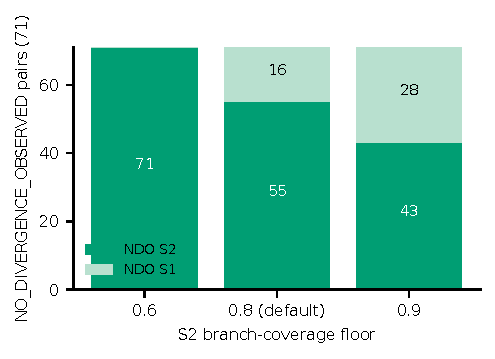
\includegraphics[width=0.92\columnwidth]{../../results/v7b_phase2_summary/figures/fig_p2_e5_floors.pdf}
\caption{E5: share of NO\_DIVERGENCE\_OBSERVED pairs labelled S2 versus S1 as the S2 branch floor varies. Verdict values are unchanged. Source: \path{results/v7b_phase2_summary/p2_consolidated_20261118_190644/consolidated.json}, key \texttt{E5}.}\label{fig:e5}
\end{figure}

\textbf{Other sensitivity and generalisation.} Repeat counts, the CPU budget and the per-run limits were not varied. Nothing supports generalisation across projects, domains, languages or platforms (Section~\ref{sec:limitations}).

\section{Runtime}\label{sec:runtime}
E6 measured a fixed 40-pair subset (seed 20261118; quotas 8/8/16/8 over the arms), 5 repetitions, sequential, one fresh process per job, on the Apple M4 Pro, \textbf{on battery power}. Both runs were flagged by the pre-registered load rule (run 1 load average 4.81 at start and 1.65 at the end; the repeat 1.44 and 2.24; transient spikes from other applications); 0 jobs failed; both runs are reported (Table~\ref{tab:e6}, Fig.~\ref{fig:e6}). V7-B's median per-pair wall time is 2.075~s against 1.310~s for B1: the median per-pair ratio is 1.595 (95\% CI $[1.584, 1.742]$) in wall time and 1.718 $[1.706, 1.844]$ in CPU time, and 1.018 $[1.014, 1.072]$ against B1+rep. V7-B therefore costs about $1.6\times$ B1, the interval excludes 1, and about as much as B1+rep. The median coefficient of variation across the five repetitions is 0.48\% (V7-B wall, run 1). Peak resident memory (tree maximum measured by the driver) has a median of about 26~MiB for V7-B and 28~MiB for B1, with a maximum of about 700~MiB for one pair; the engine does not log per-run memory. These figures are for one machine and a 40-pair subset and are not a scalability result.
\begin{table}[t]\centering\scriptsize\setlength{\tabcolsep}{3pt}
\caption{E6 runtime, 40-pair subset, 5 repetitions (V0 = default V7-B). Median per-pair wall time in seconds and median per-pair ratios with 95\% CI. Both runs were flagged by the pre-registered load rule; machine on battery power. Last column: 1-minute load average at start. Source: \path{results/v7b_phase2_summary/p2_e6_20261118_171723/timing/timing_summary.json} and \path{p2_e6b_20261118_174414/timing/timing_summary.json}.}\label{tab:e6}
\resizebox{\linewidth}{!}{%
\begin{tabular}{lrrrrrr}
\hline
Run & V0 wall & B1 wall & V0/B1 wall & V0/B1 CPU & V0/B1+rep wall & Load \\
\hline
run 1 & 2.075 & 1.310 & 1.595 [1.584, 1.742] & 1.718 [1.706, 1.844] & 1.018 [1.014, 1.072] & 4.81 \\
run 2 & 2.067 & 1.308 & 1.598 [1.586, 1.736] & 1.716 [1.706, 1.836] & 1.018 [1.015, 1.071] & 1.44 \\
\hline
\end{tabular}}
\end{table}

\begin{figure}[t]\centering
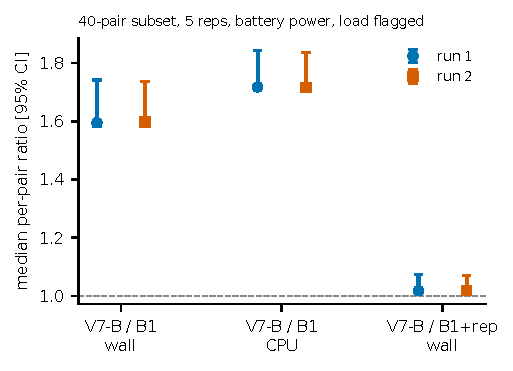
\includegraphics[width=0.92\columnwidth]{../../results/v7b_phase2_summary/figures/fig_p2_e6_overhead.pdf}
\caption{E6 median per-pair runtime ratios with 95\% CI for two runs; the dashed line is parity. Source: \path{results/v7b_phase2_summary/p2_e6_20261118_171723/timing/timing_summary.json} and \path{p2_e6b_20261118_174414/timing/timing_summary.json}.}\label{fig:e6}
\end{figure}

\section{Failure Analysis}\label{sec:failure}
This section describes observed failure modes in the development data (Tables~\ref{tab:reasons} and~\ref{tab:byarm}).
\begin{itemize}
\item \textbf{Engine gaps and conservative blocking dominate \INS{}.} Of 157 \INS{} verdicts on the driven pairs, 54 are \texttt{unmodelled\_change}, 49 \texttt{unsupported\_signature} (renamed or unsupported entries) and 40 \texttt{changed\_region\_not\_activated} (the inputs never reached the changed lines). Generator functions are not consumed and nine pairs are not driven (class units and one unsupported entry policy). The abstention rate is therefore not a measure of anything beyond engine gaps and conservative blocking on development data, and its usefulness is unshown.
\item \textbf{\texttt{unmodelled\_change} is unrefined.} Continuation lines of an executable statement are not mapped to the statement; the rule A-U1 abstains on them. Part of the 54 abstentions may be noise of the rule.
\item \textbf{\NDO{} on pairs known to differ.} 13 of 106 divergent-labelled pairs still receive \NDO{}; the battery did not reach the differing behaviour and S2 does not prevent this.
\item \textbf{Timing-dependent witness identity.} One pair (\texttt{quixbugs/longest\_common\_subsequence}) has a different witness id in E4-V0 than in E1 and E3: one input sits at the 2~s CPU limit and hit it on one side in one run (limit-asymmetric), so a later input became the witness. The verdict is unchanged, but witness identity is timing-dependent for inputs near a resource limit. Strict-key consistency is 321 of 321 between E1 and E3 and 320 of 321 between E3 and E4-V0.
\item \textbf{Label strictness.} The boundary treats the type tag as identity, so a semantics-preserving rewrite returning a boolean for an integer yields a witness; six suspect labels are excluded.
\item \textbf{Capture and determinism gaps.} Control alternation does not virtualise \texttt{datetime.now}, hash-order sensitivity is untested, and subprocess or detached-session behaviour is untested under isolation.
\end{itemize}

\section{Discussion}\label{sec:discussion}
\textbf{What the data show.} On these 258 labelled development pairs, making \NDO{} conditional on recorded sufficiency and reproducibility checks lowered the share of divergent-labelled pairs reported as ``no difference'' from 0.226 to 0.123. The reduction is \emph{entirely abstention}: all 11 of 11 pairs recovered from B1's false assurances became \INS{}, none became \DIV{}, and on the 88 divergent pairs where V7-B does not abstain, V7-B and B1 detect and miss exactly the same pairs. \textbf{Detection was not improved} (75/106 versus 82/106; a possible loss that is not significant after Holm correction). The \textbf{+10 point effect-of-interest rule is not met}. This is a calibrated-abstention result: V7-B moves some ``no difference'' answers to ``insufficient evidence'', which is the design intent, but it pays for this with an abstention rate of 0.473.

\textbf{The abstention is partly an artefact of an unrefined rule.} Between the earlier post-fix run and the current engine, abstention rose from 0.360 to 0.473 while detection and false assurance stayed unchanged, because 54 pairs now return \INS{}(\texttt{unmodelled\_change}). Of these, only three evidence packages were inspected. The increase therefore neither demonstrates a further false-assurance reduction nor shows that the rule is well calibrated, and it makes the headline abstention rate partly a property of a conservative rule awaiting refinement.

\textbf{Ablations cannot show component value.} No ablation changed any verdict, and B1+rep equals B1. Because the data contain almost no nondeterminism (1 of 312 pairs quarantined), this is an absence of opportunity, not evidence that replay, control alternation or the S2 floor are unnecessary or valuable. The same holds for E5: the floor relabels S1 and S2 without changing any verdict, so the sufficiency \emph{levels} have no demonstrated discriminating value; only the \emph{gate} (the blockers) lowers false assurance.

\textbf{Cost and evidence.} V7-B costs about $1.6\times$ the same-input baseline and about the same as the repetition-matched baseline. Verification succeeded on 828 of 828 evidence directories, but this establishes record consistency, not tamper-resistance: edits that recompute the chain are not detected.

\textbf{Relation to prior work.} Each primitive has prior art (Section~\ref{sec:related}). The defensible statement is a design-level integration whose parts are executable witnesses, an evidence-grounded insufficient outcome, a recorded change-exercise gate and typed reproducibility evidence; its measured benefit here is a lower false-assurance count obtained by abstention on non-pristine data. We make no comparison with, and no claim of improvement over, any published tool.

\section{Threats to Validity}\label{sec:threats}
\textbf{Data (internal and external).} All data are non-pristine and there is no independent holdout. QuixBugs and BugsInPy are public and widely used benchmarks, so exposure through earlier evaluations or through public sources cannot be excluded; synthetic pairs were scored by earlier systems; V7-B and its thresholds were shaped while seeing these pairs. Every result is therefore exploratory, and no result supports generalisation.

\textbf{Labels.} Divergent and no-difference labels are generator labels or a test-replay oracle; they are not adjudicated. ``Equivalent'' synthetic labels use a looser equality than the observation boundary, so a witnessed pair may be a label artefact; six suspect labels are excluded and 57 pairs are unlabelled. False assurance is relative to labels, not to verified misses. BugsInPy units are run on synthetic batteries rather than project tests.

\textbf{Statistical conclusion.} One cluster (QuixBugs, 29 divergent pairs) is large; percentile bootstrap intervals with few independent projects can undercover; pairs cluster by project; the $p$-values are descriptive. Power is too low for a confirmatory claim. The attribution statistic rests on $n=11$.

\textbf{Construct.} The sufficiency level is a coverage proxy of contested validity~\cite{inozemtseva2014coverage,just2014mut}; S2 is reachable from two inputs; no evidence shows that S1 or S2 discriminate correct from incorrect verdicts. The abstention rate reflects engine gaps and a conservative, unrefined rule more than a calibrated judgement.

\textbf{Environment and reproducibility.} One machine, one operating system (macOS) and one interpreter version; isolation is not validated; E6 was run under battery power with a load-rule flag. Determinism is incomplete (fixed hash seed never varied, \texttt{datetime.now} not virtualised) and witness identity is timing-dependent near resource limits. The E1 comparison is confounded with other engine changes.

\textbf{Evidence integrity.} The hash chain is unkeyed and not tamper-proof; a deliberate writer can produce a log that verifies; the result channel shares an address space with the evaluated program.

\textbf{Literature.} The related-work review is thematic, by one reviewer, and most statements rest on abstracts, tool-mediated reads or metadata; ``we found none'' is not a proof of absence (Section~\ref{sec:related}).

\section{Limitations}\label{sec:limitations}
\begin{itemize}
\item \textbf{Scope of the tool.} Python top-level functions in single files; user-supplied JSON inputs (no generation, no tuples, sets or objects); no classes, generators, declared renames, multi-file or repository-level changes, or non-Python code. The explorer, internal-state module and S3 are not implemented.
\item \textbf{Isolation.} macOS \texttt{sandbox-exec} only, policy flagged below the specification minimum. Linux, Docker and OS-level isolation were not implemented, tested or validated. No safe-execution or cross-platform claim.
\item \textbf{Evidence.} The chain is not tamper-proof and there is no trust anchor; \texttt{verify} executes nothing; the log contains unredacted source and inputs. Merkle log and supersession records are not implemented.
\item \textbf{Determinism.} Not complete: fixed, unvaried hash seed (hash-order sensitivity untested; E2 not run); \texttt{datetime.now} not virtualised; process ids, threads and addresses uncontrolled; timing-dependent witness identity near resource limits.
\item \textbf{Thresholds.} The 0.80 floor, repeat counts and limits are unvalidated defaults; E5 shows only that the floor relabels S1 and S2.
\item \textbf{Evaluation.} Non-pristine development data, no holdout, no adjudicated labels, no independent projects; K1 and K5 and all Phase 3 work deferred; published tools not compared; results are exploratory.
\item \textbf{Specification.} 135-rule implementation conformance is 78 conforming, 30 partially, 7 deviating, 14 not implemented, 2 unverifiable, 4 deferred to Phase 3; several user decisions (for example UD-2, the treatment of unmodelled changed lines) remain open.
\end{itemize}
Table~\ref{tab:notevaluated} lists what is not evaluated.

\section{Conclusion}\label{sec:conclusion}
V7-B implements a closed three-verdict contract for comparing two versions of a Python function, with replayable witnesses, a recorded sufficiency level on every no-difference verdict and a hash-chained evidence log with a \texttt{verify} command. In a local, exploratory Phase 2 evaluation on 321 non-pristine pairs, it reported ``no difference'' on fewer divergent-labelled pairs than same-input differential execution (13/106 versus 24/106), but only by abstaining: 11 of 11 recovered cases became \INS{}, detection was not improved (75/106 versus 82/106), the +10 point rule was not met and V7-B abstained on 122 of 258 pairs, partly through an unrefined conservative rule. Ablations changed no verdict and so cannot show component value. Isolation is macOS-only, determinism is incomplete, the evidence chain is not tamper-proof, and no published tool was compared.

The work is a design and feasibility report, not a validation. Phase 3 requires Linux isolation, real-pair feasibility (K1) and a confirmatory design (K5) with independent benchmarks and a holdout, comparison with published tools under a fair design, hash-order and seed-variation experiments, a trust anchor for the evidence log, and a refinement of the \texttt{unmodelled\_change} rule.

\section{Reproducibility and Artifact Availability}\label{sec:repro}
\textbf{Compact results} are tracked in \path{results/v7b_phase2_summary/} (per-experiment CSV and JSON, run logs, \texttt{RUN\_RECORD.md} and command scripts). \textbf{Raw evidence archives} (about 470~MB, about 27,000 files) are \emph{not} in git; they are preserved as \texttt{tar.gz} files outside the repository and identified by the sha256 sums in \path{results/v7b_phase2_summary/RAW_ARCHIVE_SHA256SUMS.txt} (seven archives: E1, E3, E4, E5, E6, E6b, E7). The artefact location is not a public repository and no long-term archive (DOI) exists yet; the repository state is branch \texttt{research/v7b-final-validation}, commit \texttt{debc4396}.

\textbf{Scripts and commands.} The E1 run uses \path{experiments/v7b/k1_spike.py} and \path{scripts/e1_analyze.py}; E3 runs the stages in \path{results/v7b_phase2_summary/p2_e3_20261118_092700/E3_COMMANDS.sh}; E4, E5 and E6 have their own \texttt{*\_COMMANDS.sh}; E6 uses \path{scripts/p2_e6_runtime.py}, E7 \path{scripts/p2_e7_verify.py} and the consolidation \path{scripts/p2_consolidate.py}. The statistics use \path{scripts/analyze_results.py} (project-cluster bootstrap $B=10000$, seed 42), \path{scripts/power_actual.py} and \path{scripts/build_dev_pairs_csv.py}. All figures and generated tables of this manuscript are produced by \path{scripts/p2_make_paper_figures.py} (\texttt{.venv/bin/python scripts/p2\_make\_paper\_figures.py}) directly from the compact results, and \path{paper/IEEE_ACCESS_INITIAL_MANUSCRIPT/scripts/check_manuscript.py} checks citations, labels, included files and table numbers. \path{paper/IEEE_ACCESS_INITIAL_MANUSCRIPT/NUMERICAL_CLAIM_VERIFICATION.md} maps each number in the abstract and results to its source file and key.

\textbf{Expected reproducibility.} Verdicts, levels, reasons and witness ids are expected to reproduce on the same platform, with the stated exception of timing-dependent witness identity near resource limits; bootstrap intervals to numeric precision; CPU and wall times only approximately. Reproduction on another operating system or interpreter version is untested. Analysis libraries are not version-pinned. This manuscript has not been compiled (\path{paper/IEEE_ACCESS_INITIAL_MANUSCRIPT/COMPILE_OVERLEAF.md}).

\bibliographystyle{IEEEtran}
\bibliography{references}
\end{document}
